\chapter{Progetto Sperimentale - SchnorrAuthApp}

% TODO: obiettivi: sicurezza, mascheramento autenticazione/registrazione

Questo capitolo è dedicato esclusivamente allo sviluppo di un sistema di autenticazione basato sul protocollo d'identificazione di Schnorr. L'obiettivo di questo progetto è di fornire un sistema di autenticazione sicuro che permetta all'utente di autenticarsi senza l'utilizzo di una password, infatti, come vedremo meglio nei paragrafi successivi, l'utente avrà bisogno solamente di uno username. Oltre a questo, ciascun utente avrà la possibilità di associare più dispositivi ad un unico account, acquisendo, in tal modo, la capacità di autenticarsi in seguito senza password dal nuovo dispositivo associato.

L'intero sistema è centralizzato in un server Python (Python Software Foundation, 2025 \textit{Python: A dynamic, open source programming
	language} \cite{python}) e un database MongoDB (MongoDB Inc. 2025 \textit{Mongodb: The developer data platform} \cite{mongodb}) usato per memorizzare le informazioni riguardo l'account di ciascun utente. A scopi didattici, è stato poi sviluppato un client Python, eseguibile da riga di comando, compatibile solo con sistemi Linux, che permette di collegarsi al server mediante socket TCP (W. Eddy, \textit{Transmission Control Protocol (TCP)} RFC 9293 \cite{rfc9293}) e stabilire una connessione client - server. Una volta stabilita la connessione, il client offre la possibilità di registrarsi, autenticarsi e, se necessario, di accoppiare un nuovo dispositivo.

Infine, è stata sviluppata un'applicazione client Android usando il framework Flutter (Google, \textit{Flutter: Build apps for any screen}, 2025 \cite{flutter}).

Il codice del server e del client Python che implmentano il funzionamento del protocollo d'identificazione di Schnorr è possibile trovarlo nel repository al seguente link: \hyperlink{https://github.com/IonutZbir/ServerClientSchnorr}{https://github.com/IonutZbir/ServerClientSchnorr}.

Il codice sorgente dell'applicazione Flutter è possibile trovarlo nel repository al seguente link: \hyperlink{https://gitlab.com/IonutZbir/SchnorrAuthApp}{https://gitlab.com/IonutZbir/SchnorrAuthApp}.

%\pagebreak
\newpage
\section{Analisi Architetturale}

Prima di procedere con la spiegazione dettagliata del funzionamento del sistema, è necessario fare le opportune analisi delle scelte architetturali, per capirne al meglio l'implementazione.

Al fine di sviluppare il sistema di autenticazione mediante protocollo d'identificazione di Schnorr, è stato definito il protocollo di comunicazione (\textbf{SAP - Schnorr-based Authentication Protocol}, analizzato successivamente nella \autoref{sec:sap}) basato sul modello classico \texttt{client-server}. Poiché è un sistema interattivo, SAP è \textbf{stateful}, ovvero è un protocollo di comunicazione che mantiene lo stato della sessione tra le richieste.

\subsection{Scelta e Definizione del Database}\label{sec:mongo}

Come menzionato prima, l'architettura sulla quale è basato il sistema è di tipo client-server, dove il client ha il ruolo di \textit{prover} mentre il server ha il ruolo di \textit{verifier}. Il database scelto è MongoDB, un database non relazionale. Si è deciso quindi di optare per MongoDB anziché un database relazionale in quanto:
\begin{itemize}
    \item \textbf{Praticità}: è più pratico in quanto i dati da memorizzare non sono molto complessi, infatti, le entità sono abbastanza elementari. Inoltre, sono documenti molto naturali da rappresentare in formato \texttt{JSON}. MongoDB, in questo senso, è perfetto, perché permette di salvare e recuperare velocemente questi documenti senza dover progettare un intero schema relazionale con tabelle, vincoli e join.
    \item \textbf{Flessibilità}: un altro punto è la flessibilità dello schema. Durante lo sviluppo del sistema di autenticazione la struttura dei dati è cambiata innumerevoli volte e, con MongoDB, questo è possibile farlo senza dover modificare una o più migrazioni \texttt{SQL}.
    \item \textbf{Semplicità}: infine, c'è l'aspetto della semplicità di integrazione con il codice. Infatti, usando Python, lavorare con dizionari e oggetti che finiscono direttamente in un documento MongoDB è molto lineare in quanto la struttura dei dizionari Python è molto simile ai documenti \texttt{JSON}.
\end{itemize}

La comunicazione tra Python e MongoDB è possibile tramite la libreria \texttt{beanie}\cite{beanie}, un \textit{Object-Document Mapper} (ODM) asincrono per MongoDB. Tale libreria si occupa di astrarre la gestione diretta dei documenti, permettendo di interagire con essi come se fossero oggetti Python, semplificando notevolmente le operazioni di lettura, scrittura e aggiornamento dei dati. I modelli di dati sono basati su \texttt{Pydantic}\cite{pydantic} un potente framework per la definizione e la validazione dei modelli, che garantisce coerenza e correttezza dei dati memorizzati nel database.

Nel progetto in esame, i modelli dei documenti sono stati dichiarati all'interno del file \texttt{server/models.py}. In questo file vengono descritte le strutture dei dati che rappresentano le diverse entità del sistema.

\begin{listing}[!ht]
\begin{minted}{python}
class PublicKey(Document):
    pk: str
    hash_pk: str
    device_name: str
    logged: bool

class User(Document):
    username: str
    public_keys: List[Link[PublicKey]]
    created_at: datetime = datetime.now()

class HashedUser(Document):
    hask_pk: str
    user: Link[User]

class Pairing(Document):
    hash_pk: str
    pk: Link[PublicKey]
    created_at: datetime
    expiry: datetime 
    
    @property
    def is_expired(self):
        return datetime.now() > self.expiry
\end{minted}
\caption{Definizione dei modelli all'interno del file \texttt{server/models.py}}
\label{cod:schema_db}
\end{listing}



\newpage

\newsavebox{\lstone}
\newsavebox{\lsttwo}
\newsavebox{\lstthree}
\newsavebox{\lstfour}

\begin{lrbox}{\lstone}
\begin{minipage}{0.46\textwidth}
\begin{minted}[escapeinside=||,fontsize=\small]{json}
{
  "_id": "<ObjectId1>"|\tikzmark{A}|,
  "username": "Ionut",
  "public_keys":["<ObjectId3>"]|\tikzmark{C}|,
  "created_at": "2025-09-09|16:00"
}
\end{minted}
\end{minipage}
\end{lrbox}

\begin{lrbox}{\lsttwo}
\begin{minipage}{0.45\textwidth}
\begin{minted}[escapeinside=||,fontsize=\small]{json}
{
  "_id": "<ObjectId2>",
  |\tikzmark{B}|"user": "<ObjectId1>",
  "hash_pk": "c1cb6eff..."
}
\end{minted}
\end{minipage}
\end{lrbox}

\begin{lrbox}{\lstthree}
\begin{minipage}{0.45\textwidth}
\begin{minted}[escapeinside=||,fontsize=\small]{json}
{
  |\tikzmark{D}|"_id": "<ObjectId3>",
  "pk": "0xe109e1a50581...",
  "hash_pk": "be257ea8a...",
  "device_name": "ASUS Linux...",
  "logged": false
}
\end{minted}
\end{minipage}
\end{lrbox}

\begin{lrbox}{\lstfour}
\begin{minipage}{0.46\textwidth}
\begin{minted}[escapeinside=||,fontsize=\small]{json}
{
  "_id": "<ObjectId4>",
  "pk": "<ObjectId3>"|\tikzmark{E}|,
  "hash_pk": "0xe864e1f...",
  "created_at": "2025-09-09|17:39",
  "expiry": "2025-09-09|17:49"
}
\end{minted}
\end{minipage}
\end{lrbox}

\renewcommand{\arraystretch}{1.8}

\begin{tabularx}{\textwidth}{X@{\hspace{2cm}}X}
User document \vspace{1mm} \newline
\fbox{\usebox{\lstone}} &
HashedUser document \vspace{1mm} \newline
\fbox{\usebox{\lsttwo}} \\[1cm]

Pairing document \vspace{1mm} \newline
\fbox{\usebox{\lstfour}} &
PublicKey document \vspace{1mm} \newline
\fbox{\usebox{\lstthree}}
\end{tabularx}

\begin{figure}[!ht]
    \begin{tikzpicture}[remember picture,overlay,>=stealth]
        % frecce
        \draw[<->,thick, blue](A) -- (B);
        \draw[<->,thick, blue](C) -- (D);
        \draw[<->,thick, blue](E) -- (D);
    \end{tikzpicture}
    \caption{Database Schema}
    \label{fig:schema_db}
\end{figure}

\hrulefill


Come mostrato in \autoref{fig:schema_db} e come definito nel \autoref{cod:schema_db}, lo schema del database consiste di 3 documenti:
\begin{itemize}
    \item \texttt{\textbf{User}}: è il documento principale nel quale sono memorizzate le informazioni di ciascun utente, come lo username e la lista delle chiavi pubbliche associate ad esso.
    \item \texttt{\textbf{HashedUser}}: rappresenta una mappatura \texttt{hash\_pk} $\rightarrow$ \texttt{user}, utile per identificare in modo rapido l'utente che sta provando ad autenticarsi usando l'hash della sua chiave pubblica. Infatti, al momento dell'autenticazione, il client invierà oltre allo username anche l'hash della chiave pubblica per identificare facilmente e in modo univoco l'utente che prova ad autenticarsi.
    \item \texttt{\textbf{PublicKey}}: contiene le informazioni di ciascuna chiave pubblica registrata, il dispositivo sul quale è memorizzata, il suo hash e infine un campo booleano \texttt{logged}.
    \item \texttt{\textbf{Pairing}}: viene aggiunto un nuovo record quando un dispositivo \textit{slave} chiede di essere abbinato ad un account. È un documento di appoggio che permette di eseguire l'accoppiamento dei dipositivi.
\end{itemize}

\subsection{Calcolo dell'Hash delle Chiavi Pubbliche}\label{sec:hash_compute}
L'hash viene calcolato usando un algoritmo crittografico di hash (ad esempio \texttt{SHA-256} discusso nella \autoref{sec:sha}), che restituisce una stringa di lunghezza fissa. Questo valore viene poi memorizzato nel campo \texttt{hash\_pk} e utilizzato come indice per risalire rapidamente all'utente associato, senza dover trasmettere direttamente la chiave pubblica completa ogni volta che l'utente si prova ad autenticare. Infatti, in questo modo la chiave pubblica viene comunicata al server una sola volta in fase di registrazione.
\begin{listing}[!ht]
    \begin{minted}{Python}
    import hashlib
    def hash_public_key_SHA256(public_key: int) -> 'hashlib.Hash':
        pk_len_bits = public_key.bit_length()
        pk_bytes = public_key.to_bytes((pk_len_bits + 7) // 8)
        return hashlib.sha256(pk_bytes) 
    \end{minted}
\caption{Calcolo dell'hash della chiave pubblica in Python}
\end{listing}

\subsection{Salvataggio della Chiave Segreta in Locale}\label{sec:key_manager}

Un' ulteriore scelta architetturale è stata quella di salvare su file locale la chiave privata di ciascun account registrato dal dispositivo. Nello specifico, andremo a discutere quale strategia è stata applicata per salvare le chiavi private su dispositivi Linux e perché tale strategia è sicura.

Quando l'utente si registra da un dispositivo Linux, la chiave viene salvata all'interno di un file \texttt{user\_privkey.pem} nella directory \texttt{/home/user/.schnorr}. Inoltre, il client ha la possibilità di impostare una password, la quale verrà poi usata per derivare la chiave di cifratura dell' algoritmo di cifratura a blocchi \texttt{AESGCM} discusso nella \autoref{sec:aes}. Se l'utente non imposta una password, allora la chiave viene salvata in chiaro senza applicare nessun algoritmo di cifratura.

Nell'implementazione Python del client, il modulo che si occupa di caricare e salvare la chiave su file locale si trova in \texttt{client/utils.key\_manager.py}. Un'implementazione simile a quella reale si trova in Appendice, nella \autoref{sec:key_manager}.

\subsection{SchnorrProver e SchnorrVerifier}\label{sec:class_schnorr}

Come discusso all'inizio del capitolo, il client assume il ruolo di \textit{prover}, mentre il server ricopre quello di \textit{verifier}. In particolare, ogni client istanzia un oggetto della classe \texttt{SchnorrProver} e, per ciascuna fase del protocollo, utilizza la chiave privata $\alpha$, la coppia di chiavi temporanee $(\alpha_t, u_t)$ — dove $u_t$ rappresenta il \textit{commitment} inviato al \textit{verifier} — e la risposta $\alpha_z$, calcolata dopo aver ricevuto la \textit{challenge}. Sul lato server, per ogni client in ingresso viene creata una task\footnote{Il server utilizza il modulo \texttt{asyncio} per la gestione concorrente, basata su \textit{task} asincroni piuttosto che su \textit{thread} nativi.} insieme a un'istanza della classe \texttt{SchnorrVerifier}. Le due classi hanno il ruolo di centralizzare le operazione aritmetiche necessarie per il corretto funzionamento del protocollo d'identificazione e per la firma digitale di Schnorr. In Appendice, nella \autoref{sec:schnorr_classi} è mostrata un'implementazione semplificata delle due classi insieme ad un esempio di funzionamento.

\section{Funzionamento del Protocollo SAP}\label{sec:sap}

Il funzionamento di SAP è diviso in 3 fasi fondamentali: la prima consiste in una fase di handshake, nella quale client e server concordano i parametri necessari alla comunicazione, la seconda è la fase di registrazione nella quale il client si registra presso il server e la terza è la fase di autenticazione che segue nei minimi dettagli il protocollo di Schnorr. 


\subsection{Fase di Handshake}
Una volta stabilita la connessione tra client e server ha luogo una fase di \textit{handshake}. In questa fase, i due attori concordano i parametri necessari per l'autenticazione mediante protocollo d'identificazione di Schnorr, ossia, il gruppo matematico da utilizzare per i calcoli crittografici. Questo scambio iniziale consente di sincronizzare client e server, garantendo che entrambi operino con gli stessi valori di riferimento prima di procedere con le successive fasi del protocollo.

Sia client che server dispongono di una lista di gruppi crittografici con i quali sono abilitati a lavorare. Il server, al momento della connessione di un client, invia una lista dei gruppi crittografici a cui è abilitato per i calcoli matematici. Il client verifica, poi, se dispone dei gruppi ricevuti dal server e sceglie il primo disponibile. Se non dispone di nessun gruppo, invia un messaggio al server comunicando che la sincronizzazione non può avvenire e chiude la connessione. Per la scelta dei gruppi crittografici da utilizzare è stato adoperato il seguente standard \textit{RFC 3526} \cite{rfc3526}, nel quale è presente una lista di gruppi crittografici standardizzati.


La fase di \textit{handshake} consiste nei seguenti passaggi, come mostrato in \autoref{fig:handshake}.

\begin{enumerate}
	\item Il client invia al server un messaggio \mintinline{json}|{"type":"HANDSHAKE_REQ"}|;
	\item {
    Il server risponde, poi, al client con un messaggio del tipo
    \begin{center}
      \begin{minted}{json}
        {
            "type":"HANDSHAKE_RES",
            "crypto_groups":["modp-2048", "modp-4096"]
        }
      \end{minted}
    \end{center}
    }
	\item Il client verifica se è abilitato ad usare almeno uno dei gruppi ricevuti dal server e ne sceglie uno, ad esempio il primo disponibile, e lo invia al server come
	\begin{center}
      \begin{minted}{json}
        {
            "type":"HANDSHAKE_OK",
            "group_id":"modp-4096"
        }    
	    \end{minted}
	\end{center}
	Se, invece, non è abilitato ad usare nessuno dei gruppi inviati dal server, allora risponde con \mintinline{json}|{"type":"HANDSHAKE_NOK"}| e chiude la connessione.
	\item Il server riceve il gruppo crittografico dal client e lo imposta per eseguire tutti i calcoli matematici necessari per il corretto funzionamento del protocollo SAP.
\end{enumerate}

\begin{figure}[!ht]
\centering
    \begin{tikzpicture}[ lifeline/.style={thick}, arrow/.style={-{Stealth[length=6pt,width=6pt]}, thick}, msg/.style={midway, fill=white, font=\small, inner sep=2pt, align=center} ] % Nodi principali 
	\node (client) {Client}; \node[right=6cm of client] (server) {Server}; 
	% Linee verticali (lifelines)
	\draw[lifeline] (client.south) -- ++(0,-6);
	\draw[lifeline] (server.south) -- ++(0,-6); 
	% Messaggi del 3-way handshake 
				
	% 1. HANDSHAKE REQ
	\draw[arrow] ($(client.south)+(0,-0.5)$) -- ($(server.south)+(0,-0.5)$) node[msg, above] {\mintinline{json}|"type":"HANDSHAKE_REQ"|};
	% 2. HANSHAKE RES 
	\draw[arrow] ($(server.south)+(0,-2)$) -- ($(client.south)+(0,-2)$) node[msg, above, align=left, text width=6cm] {
    \begin{minted}[fontsize=\scriptsize]{json}
            "type":"HANDSHAKE_RES", 
            "crypto_groups":["modp-4096"]
      \end{minted}
    };
	% 3. HANDSHAKE OK/NON 
	\draw[arrow] ($(client.south)+(0,-3.5)$) -- ($(server.south)+(0,-3.5)$) node[msg, above, align=left, text width=6cm] {
    \begin{minted}[fontsize=\scriptsize]{json}
            "type":"HANDSHAKE_OK",
            "group_id":"modp-4096"
      \end{minted}
    };
	% --- ramo NOK ---
	\draw[arrow, red, dashed] ($(client.south)+(0,-5)$) -- ($(server.south)+(0,-5)$)
	node[msg, above] {\mintinline{json}|"type":"HANDSHAKE_NOK"|};		
    \end{tikzpicture}
    \caption{Interazione tra client e server durante la fase di handshake}
    \label{fig:handshake}
    \end{figure}

\noindent\hrulefill

\newpage

\subsection{Fase di Registrazione/Autenticazione}

Una volta impostati i parametri stabiliti nella fase di handshake, client e server sono ora pronti per poter comunicare mediante \textbf{SAP}. Adesso l'utente si può autenticare/registrare sul server digitando uno username, qualsiasi esso sia. Uno degli obiettivi principali, oltre alla sicurezza di questo sistema d'autenticazione client-server, è quello di mascherare all'utente finale la fase di \textit{registrazione} al server. L'utente non deve essere a conoscenza del fatto che si stia registrando al server ma deve sapere soltanto che si sta autenticando. Infatti, l'unica opzione di cui dispone l'utente è quella di accedere mediante username. Spetta, quindi, al sistema determinare se procedere o meno con la registrazione dell'account. 

La fase di autenticazione prevede che l'utente inserisca il proprio username, dopodiché il client software proverà a caricare dal disco\footnote{La modalità con il quale il sistema cifra e salva poi su disco la chiave privata dell'utente viene discussa nella \autoref{sec:key_manager}} la chiave privata $\alpha$. Poiché uno degli obiettivi principali di questo sistema di autenticazione è di nascondere all'utente finale la fase di registrazione, questa avviene quando il file contenente la chiave privata non è presente sul disco e, in tal caso, si procede con la registrazione del nuovo account.

In seguito, verrà mostrato un esempio di funzionamento delle fasi registrazione e autenticazione al fine di comprenderlo al meglio. Supponiamo che l'utente \textit{Ionut} si voglia autenticare dal suo dispositivo portatile \texttt{LENOVO}, il client prova a leggere dal disco la chiave privata di \texttt{Ionut}, allora:

\begin{itemize}
	\item Se il file con la chiave non esiste, allora significa che \texttt{Ionut} non è registrato, o meglio, non è presente la sua chiave in locale, in quanto sul server potrebbe già essere presente un account registrato con lo username \texttt{Ionut}. Infatti, il server per distinguere due utenti con lo stesso username identifica in modo univoco ciascun utente mediante un identificatore univoco generato in automatico da MongoDB. In alternativa, si potrebbe utilizzare uno \texttt{uuid} generato al momento della registrazione, ma per semplicità è stato scelto di usare l'object id di Mongo. A questo punto, il client genera la sua coppia di chiavi, $(\alpha,\ u := g^\alpha)$ richiamando il metodo \texttt{SchnorrProver.genKeys()}, come discusso nella \autoref{sec:class_schnorr}. La chiave privata $\alpha$ verrà memorizzata su file locale, mentre la chiave pubblica $u$ verrà invita, in seguito, al server insieme al nome del dispositivo da cui si è effettuata la registrazione, in un messaggio di tipo:
	      \begin{center}
	      	\begin{minted}[escapeinside=||, mathescape=true]{json}
            {
                "type":"REGISTRATION_REQ",
                "username":"Ionut",
                "public_key": |$u$|,
                "device": "LENOVO"
            }
	      	\end{minted}
	      \end{center}
	      Ricevuta la richiesta dal client, il server memorizza all'interno del database il nuovo utente, creando un nuovo oggetto \texttt{User} e \texttt{PublicKey}. Infine, crea un nuovo oggetto \texttt{HashedUser} mappando in questo modo l'hash della chiave pubblica al nuovo utente (\texttt{SHA256($u$) $\rightarrow$  username}), facilitando l'operazione di ricerca durante la fase di autenticazione\footnote{Per maggiori dettagli, vedere \autoref{sec:mongo}}. A questo punto, il server risponde al client comunicando l'avvenuta registrazione con successo dell'account.
          \begin{center}
	      	\begin{minted}[escapeinside=||, mathescape=true]{json}
            {"type":"REGISTERED", "username":"Ionut"}
	      	\end{minted}
	      \end{center}
	\item {Se, invece, il file con la chiave privata esiste, allora il client procede con la fase di autenticazione. Dunque, genera le chiavi temporanee $(\alpha_t,\ u_t := g^{\alpha_t})$, ricordando che $u_t$ rappresenta il \textit{commitment}, e invia quest'ultima al server insieme all' hash della sua vera chiave pubblica $u$.
		\begin{center}
			\begin{minted}[escapeinside=||, mathescape=true]{json}
            {
                "type":"AUTH_COMMITMENT",
                "username":"Ionut",
                "public_key_temp": |$u_t$|,
                "pk_hash": |$\texttt{SHA265}(u)$|
            }
			\end{minted}
		\end{center}
		Ricevuto il messaggio contenente il commitment, il server usa l'hash della chiave pubblica per interrogare il database, così da individuare l'utente corrispondente. Se l'utente esiste, allora, procede con la generazione della challenge $c$ e la invia al client.
		\begin{center}
			\begin{minted}[escapeinside=||, mathescape=true]{json}
            {
                "type":"AUTH_CHALLENGE",
                "challenge": |$c$|
            }
			\end{minted}
		\end{center}
		Ricevuta la challenge, il client calcola la \textit{response} $\alpha_z = \alpha_t + \alpha c$, comunicandola al server.
		\begin{center}
			\begin{minted}[escapeinside=||, mathescape=true]{json}
            {
                "type":"AUTH_RESPONSE",
                "response": |$\alpha_z$|
            }
			\end{minted}
		\end{center}
		A questo punto, il server (verifier), è in possesso di tutti i parametri necessari per passare alla verifica del client (prover). Per ogni chiave pubblica registrata presso l'utente \texttt{Ionut}\footnote{Ad ogni utente possono corrispondere una o più chiavi pubbliche, in quanto ciascun utente ha la possibilità di associare più dispositivi o addirittura unire più account.}, richiama il metodo \texttt{SchnorrVerifier.check(res)}. Se dà esito positivo, allora comunica al client che è stato autenticato con successo (\mintinline{json}|{"type": "AUTH_ACCEPTED"}|), altrimenti, se non viene autenticato viene inviato un messaggio (\mintinline{json}|{"type": "AUTH_REJECTED"}|).
	}
\end{itemize}

\begin{figure}[!ht]
\centering
    \begin{tikzpicture}[ lifeline/.style={thick}, arrow/.style={-{Stealth[length=6pt,width=6pt]}, thick}, msg/.style={midway, fill=white, font=\small, inner sep=2pt, align=center} ] % Nodi principali 
	\node (client) {Client};
    \node[right=8cm of client] (server) {Server}; 
	% Linee verticali (lifelines)
	\draw[lifeline] (client.south) -- ++(0,-10);
	\draw[lifeline] (server.south) -- ++(0,-10); 
	% Messaggi del 3-way handshake 
				
	% 1. COMMITMENT
	\draw[arrow] ($(client.south)+(0,-2)$) -- ($(server.south)+(0,-2)$) node[msg, above, align=left, text width=6cm] {
    \begin{minted}[escapeinside=||, mathescape=true]{json}
        "type":"AUTH_COMMITMENT",
        "username":"Ionut",
        "public_key_temp": |$u_t$|,
        "pk_hash": |$\texttt{SHA265}(u)$|
    \end{minted}
    };
	% 2. CHALLENGE
	\draw[arrow] ($(server.south)+(0,-4)$) -- ($(client.south)+(0,-4)$) node[msg, above, align=left, text width=6cm] {
    \begin{minted}[escapeinside=||, mathescape=true]{json}
        "type":"AUTH_CHALLENGE",
        "challenge": |$c$|
    \end{minted}
    };
	% 3. RESPONSE
	\draw[arrow] ($(client.south)+(0,-6)$) -- ($(server.south)+(0,-6)$) node[msg, above, align=left, text width=6cm] {
    \begin{minted}[escapeinside=||, mathescape=true]{json}
        "type":"AUTH_RESPONSE",
        "response": |$\alpha_z$|
    \end{minted}
    };
	% 4. ACCEPT/VERIFY
	\draw[arrow] ($(server.south)+(0,-8)$) -- ($(client.south)+(0,-8)$) node[msg, above, align=left, text width=6cm] {
    \begin{minted}[escapeinside=||, mathescape=true]{json}
        "type":"AUTH_ACCEPTED"
    \end{minted}
    };
    \draw[arrow, red, dashed]($(server.south)+(0,-9.5)$) -- ($(client.south)+(0,-9.5)$) node[msg, above, align=left, text width=6cm] {
    \begin{minted}[escapeinside=||, mathescape=true]{json}
        "type":"AUTH_REJECTED"
    \end{minted}
    };
    \end{tikzpicture}
    \caption{Interazione tra client e server durante la fase di autenticazione}
    \label{fig:auth}
    \end{figure}

\noindent\hrulefill

\newpage

\subsection{Processo di Accoppiamento di un Dispositivo}

Il principale svantaggio di un sistema di autenticazione \textit{passwordless} risiede proprio nell'assenza della password, in quanto la password/chiave privata è device/client-dependent. Di conseguenza, se l'utente dovesse perdere la propria chiave privata (ad esempio a seguito di una formattazione o dell'eliminazione accidentale del file che la contiene) il suo account risulterebbe inaccessibile, non potendo più autenticarsi al server. 
Una soluzione valida per mitigare questo problema è di offrire la possibilità agli utenti di poter associare più dispositivi allo stesso account, in questo modo, anche in caso di perdita della chiave privata su un dispositivo, sarebbe comunque possibile accedere tramite un altro.

L'idea generale del meccanismo di associazione è quella di impiegare la firma digitale di Schnorr\footnote{Per maggiori dettagli consultare la \autoref{sec:sig_schnorr}.} nella fase di conferma. Quando un utente intende associare un nuovo dispositivo (\textit{slave}), la procedura di accoppiamento deve essere confermata tramite un dispositivo già autenticato (\textit{master}).

In pratica, al momento della generazione della coppia di chiavi da parte dello slave, la chiave pubblica viene codificata in un \texttt{qr\_code} e mostrata a schermo.
Se il dispositivo master è mobile, l'utente può semplicemente scansionare il \texttt{qr\_code}, inviando al server la chiave pubblica insieme alla relativa firma. La situazione si complica invece quando il dispositivo master è un desktop: in assenza di un lettore di \texttt{qr\_code}, l'utente è costretto a inserire manualmente la chiave pubblica visualizzata, con un impatto negativo sulla user experience, poiché digitare una chiave pubblica risulta scomodo ed soggetto ad errori.

Per migliorare la user experience anche in questo scenario, si è reso necessario definire un formato alternativo per la stringa da inserire: le opzioni considerate sono state un token generato casualmente oppure una sequenza di parole in italiano.

La soluzione preferita è quella basata su una sequenza di parole, implementata mediante lo standard \texttt{BIP-39} \textit{(Bitcoin Improvement Proposal)}\cite{BIP39}. Questo \texttt{BIP} definisce l'utilizzo di un codice mnemonico, ossia una frase composta da parole di facile memorizzazione, originariamente pensata per la generazione di \textit{wallet} deterministici. Nel nostro caso, non viene generata entropia, bensì si utilizzano direttamente i bit della chiave pubblica. Tali bit vengono suddivisi in blocchi da 11, ciascuno dei quali rappresenta un numero intero compreso tra 0 e 2047, usato come indice all'interno di una lista predefinita di 2048 parole.

Tuttavia, questo approccio non risulta pratico: la codifica di una chiave pubblic, la cui lunghezza può variare da 1536 a 4096 bit, a seconda del gruppo crittografico utilizzato, genererebbe infatti una frase mnemonica composta da circa 100–300 parole, compromettendo seriamente la \textit{user experience}.
Per ovviare a questo problema, si è scelto di adottare un codice mnemonico molto più compatto, composto da una decina di parole, facilmente memorizzabile e semplice da comunicare anche verbalmente.
Inoltre, si è previsto di integrare un sistema di autocompletamento, sfruttando il fatto che la lista di parole definita dallo standard \texttt{BIP-39} è ordinata alfabeticamente. Ciò consente un recupero delle parole più efficiente, ad esempio tramite ricerca binaria invece che lineare, e permette anche l'utilizzo di strutture dati come i \texttt{trie} per ottenere una migliore compressione. 

Pertanto, anziché codificare direttamente l’intera chiave pubblica, essa viene prima sottoposta alla funzione di hash \texttt{SHA-256} e successivamente ridotta a 160 bit tramite l'algoritmo \texttt{RIPEMD-160}.
L'intero risultato di 160 bit viene quindi utilizzato per generare la frase mnemonica, che risulta composta da circa 15 parole. Questa scelta consente di ottenere un buon compromesso tra sicurezza e usabilità, mantenendo la frase sufficientemente compatta da poter essere ricordata e comunicata con facilità, senza rinunciare a un adeguato livello di protezione crittografica.

\begin{listing}[!ht]
    \begin{minted}{Python}
                from Crypto.Hash import RIPEMD160
                hash_pk = hash_public_key_SHA256(pk)
                ripemd160_pk = RIPEMD160.new()
                ripemd160_pk.update(hash_pk.digest())
    \end{minted}
\caption{Hash della chiave pubblica con \texttt{RIPEMD-160}}
\end{listing}

Con questo meccanismo, il dispositivo slave invia al server la propria chiave pubblica. Il dispositivo master, invece, ricava il medesimo prefisso a partire dalla sequenza di parole e lo trasmette al server accompagnato dalla firma.
Una volta ricevuto il messaggio dal master, il server ne verifica la firma e, se valida, associa la chiave pubblica all'account dell'utente, completando l'aggiunta del dispositivo slave.

In particolare, quando il server riceve la richiesta di associazione dal dispositivo slave, crea un nuovo oggetto \texttt{Pairing}, contenente a sua volta un oggetto \texttt{PublicKey}, insieme all'hash calcolato con \texttt{RIPEMD-160} e lo memorizza nel database. 

Successivamente, alla ricezione del messaggio di conferma dal master, esegue la verifica della firma tramite il metodo \texttt{SchnorrVerifier.verify\_sign(sign, message)}, dove \texttt{sign} è la firma $\sigma = (u_t, \alpha_z)$ inviata dal client master e \texttt{message} rappresenta l'hash della chiave pubblica.
Se la verifica fallisce, il server invia a entrambi i client un messaggio \mintinline{json}|{"type": "ASSOC_REJECTED"}|. In caso contrario, interroga il database utilizzando l'hash per recuperare l'oggetto \texttt{Pairing} precedentemente generato e ottenere la chiave pubblica del dispositivo slave. Se l'oggetto esiste, aggiorna l'account dell'utente inserendo la nuova chiave pubblica.

\newpage

\begin{figure}[!ht]
\centering
    \begin{tikzpicture}[ lifeline/.style={thick}, arrow/.style={-{Stealth[length=6pt,width=6pt]}, thick}, msg/.style={midway, fill=white, font=\small, inner sep=2pt, align=center} ] % Nodi principali 
	\node (slave) {Client-Slave};
    \node[right=5cm of client] (server) {Server}; 
	\node[right=5cm of server] (master) {Client-Master};
	% Linee verticali (lifelines)
	\draw[lifeline] (slave.south) -- ++(0,-8);
	\draw[lifeline] (server.south) -- ++(0,-8); 
	\draw[lifeline] (master.south) -- ++(0,-8);
	
	\draw[arrow] ($(slave.south)+(0,-2.5)$) -- ($(server.south)+(0,-2.5)$) node[msg, above, align=left, text width=6cm] {
    \begin{minted}[escapeinside=||, mathescape=true]{json}
    "type": "ASSOC_REQ",
    "device": "LENOVO",
    "pk": |$u$|,
    \end{minted}
    };
    \draw[arrow] ($(master.south)+(0,-4.5)$) -- ($(server.south)+(0,-4.5)$) node[msg, above, align=left, text width=6cm] {
    \begin{minted}[escapeinside=||, mathescape=true]{json}
    "type": "ASSOC_CONFIRM",
    "public_key_temp": |$u_t$|,
    "response": |$\alpha_z$|,
    "message": |$\texttt{wordsToHash(words)}$|
    \end{minted}
    };
    \draw[arrow] ($(server.south)+(0,-6)$) -- ($(slave.south)+(0,-6)$) node[msg, above, align=left, text width=6cm] {
    \begin{minted}[escapeinside=||, mathescape=true]{json}
    "type": "ASSOC_ACCPTED",
    \end{minted}
    };
    \draw[arrow] ($(server.south)+(0,-6)$) -- ($(master.south)+(0,-6)$) node[msg, above, align=left, text width=6cm] {
    \begin{minted}[escapeinside=||, mathescape=true]{json}
    "type": "ASSOC_ACCPTED",
    \end{minted}
    };
    \draw[arrow, red, dashed]($(server.south)+(0,-7.5)$) -- ($(master.south)+(0,-7.5)$) node[msg, above, align=left, text width=6cm] {
    \begin{minted}[escapeinside=||, mathescape=true]{json}
        "type":"ASSOC_REJECTED"
    \end{minted}
    };
    \draw[arrow, red, dashed]($(server.south)+(0,-7.5)$) -- ($(slave.south)+(0,-7.5)$) node[msg, above, align=left, text width=6cm] {
    \begin{minted}[escapeinside=||, mathescape=true]{json}
        "type":"ASSOC_REJECTED"
    \end{minted}
    };
    \end{tikzpicture}
    \caption{Interazione tra slave, master e server durante il processo di accoppiamento.}
    \label{fig:assoc}
    \end{figure}

\noindent\hrulefill

\newpage

\section{Applicazione Client Flutter}

Nelle sezioni precedenti è stato illustrato il funzionamento del protocollo \textbf{SAP}, con particolare attenzione allo scambio di messaggi tra client (prover) e server (verifier). Finora il client considerato era sviluppato in Python ed eseguibile da linea di comando esclusivamente su sistemi Linux. Per rendere l'utilizzo più accessibile e intuitivo, si è scelto di realizzare un'applicazione con interfaccia grafica, sviluppata in Flutter \cite{flutter}.

La scelta di Flutter è motivata soprattutto dal fatto che si tratta di un framework multipiattaforma: consente infatti di scrivere il codice in un unico linguaggio (Dart \cite{dart}) e successivamente generare l'applicazione per diversi ambienti, come Android per dispositivi mobile e Linux, Windows per dispositivi desktop.

Dal punto di vista dell'esperienza utente, l'app è stata progettata per risultare semplice e immediata: l'accesso avviene inserendo unicamente lo username, dopodiché l'interfaccia mostra lo stato della connessione e 'elenco dei dispositivi già associati all'account. L'aggiunta di un nuovo dispositivo avviene in maniera differente a seconda della piattaforma utilizzata come master: se si tratta di un dispositivo mobile, è possibile effettuare l'accoppiamento tramite la scansione del QR code generato dal dispositivo slave; se invece il master è un computer desktop, è stato previsto un sistema di autocompletamento che semplifica e velocizza la procedura di associazione.

% Parlare anche di f-droid
\subsection{F-Droid}
Un aspetto importante nello sviluppo dell'app è stato quello di garantirne la piena compatibilità con le linee guida di \textbf{F-Droid} \cite{fdroid}, il principale repository di applicazioni \textit{Free and Open Source Software (FOSS)} per dispositivi Android. F-Droid si distingue dagli store tradizionali perché distribuisce esclusivamente software libero, privo di componenti proprietarie, tracciamenti occulti o dipendenze che possano compromettere la trasparenza e la libertà dell'utente. Ogni applicazione pubblicata deve rispettare criteri rigorosi, tra cui la disponibilità del codice sorgente, la possibilità di verificarne e ricompilarne in maniera indipendente i binari, e l'assenza di meccanismi pubblicitari o sistemi di tracking.

L'applicazione sviluppata soddisfa pienamente questi requisiti sotto diversi punti di vista. Anzitutto, l'intero codice sorgente è reso disponibile pubblicamente su \texttt{GitLab}, piattaforma web open source per la gestione collaborativa di repository \texttt{Git}. Ciò consente non solo la condivisione e il versionamento del codice, ma anche la possibilità per chiunque di ispezionarlo e verificarne il corretto funzionamento \footnote{Repository GitLab: \url{https://gitlab.com/IonutZbir/SchnorrAuthApp}}. Inoltre, tutte le librerie e i pacchetti impiegati sono anch'essi open source e reperibili in repository pubblici, garantendo così la totale trasparenza dell'intera catena di dipendenze.
 Particolare attenzione è stata rivolta anche alla gestione dei dati dell'utente: non vengono raccolte informazioni personali\footnote{Infatti, l'unico dato dell'utente che viene conservato sul server è lo \textit{username}; di conseguenza, ciascun utente ha la piena libertà di scegliere il nome con cui desidera essere identificato all'interno dell'applicazione.}
 né inviati metadati a terze parti, in linea con il principio di minimizzazione dei dati promosso da F-Droid. Infine, l'assenza di sistemi pubblicitari o meccanismi di profilazione assicura che l'app rimanga uno strumento sicuro e rispettoso della privacy.

Grazie a queste caratteristiche, l'app non solo soddisfa i requisiti minimi per una distribuzione su F-Droid, ma incarna a pieno i valori del software libero: trasparenza, sicurezza, rispetto della privacy e possibilità di revisione comunitaria.

In aggiunta, la struttura della repository deve rispettare i requisiti stabiliti da F-Droid, comprendendo i metadati necessari all'applicazione. A tal fine, si è deciso di adottare l'organizzazione standard compatibile con \textit{fastlane}, così da garantire una gestione coerente e facilmente integrabile nel processo di distribuzione \footnote{Per maggiori dettagli, visitare: \url{https://f-droid.org/en/docs/All_About_Descriptions_Graphics_and_Screenshots/}}.

\subsection{Livelli di Sicurezza}

Dal momento che la chiave segreta viene conservata localmente sul dispositivo, per assicurarne la protezione è stata prevista la sua cifratura (per ulteriori dettagli si rimanda alla \autoref{sec:key_manager}). L'accesso alla chiave avviene quindi tramite l'inserimento di una password (PIN); sui dispositivi mobili, in alternativa, è possibile sbloccarla utilizzando l'autenticazione biometrica tramite impronta digitale.

In particolare, sono stati implementati due livelli di sicurezza:

\begin{enumerate}[label={}]
    \item \textbf{Livello 1 di Sicurezza} – L'utente può decidere se autenticarsi tramite PIN oppure tramite impronta digitale. Nel caso in cui venga scelta l'opzione biometrica, al primo avvio dell'app viene generata in automatico una password di 32 caratteri, che viene memorizzata localmente sfruttando la libreria Flutter \texttt{flutter\_secure\_storage}. L'impronta digitale ha quindi il solo scopo di sbloccare ogni tal volta la password utilizzata per la cifratura della chiave segreta.
    \item \textbf{Livello 2 di Sicurezza} - Poiché l'impiego di un PIN scelto direttamente dall'utente (ad esempio sequenze banali come 1234) non garantisce un livello di sicurezza adeguato, l'applicazione mette a disposizione un secondo livello di protezione. In questo caso viene utilizzata una password di 32 caratteri generata in modo casuale, analoga a quella prevista nel livello 1 quando si adotta l'autenticazione biometrica. Pertanto, se l'utente decide di inserire manualmente un PIN (nel caso in cui il dispositivo è desktop oppure il dispositivo mobile non dispone di autenticazione biometrica), ciò che in realtà deve digitare è la password generata dall'app. Il principale svantaggio di questa soluzione risiede nel fatto che l'utente dovrebbe ricordare una stringa lunga e complessa; per superare tale problema si è adottato lo stesso approccio previsto per la codifica della chiave privata durante la fase di associazione. In particolare, la password viene convertita in una sequenza mnemonica, che viene mostrata all'utente e che egli è invitato a conservare con cura, poiché rappresenta la codifica leggibile della password generata.

\end{enumerate}

\subsection{Interfaccia Grafica}

Per completare la descrizione dell'applicazione sviluppata, si ritiene utile mostrare alcune schermate rappresentative dell'interfaccia grafica. Queste immagini hanno lo scopo di fornire al lettore una visione concreta delle funzionalità principali e del flusso d'uso, mettendo in evidenza come le scelte progettuali discusse nei paragrafi precedenti siano state tradotte in una GUI semplice e intuitiva. Le figure che seguono illustrano i passaggi fondamentali: dalla fase di registrazione/accesso, alla visualizzazione dello stato della connessione e dei dispositivi associati, fino alla procedure di accoppiamento e conferma.

\begin{figure}[h!]
    \centering
    \begin{minipage}{0.45\textwidth}
        \centering
        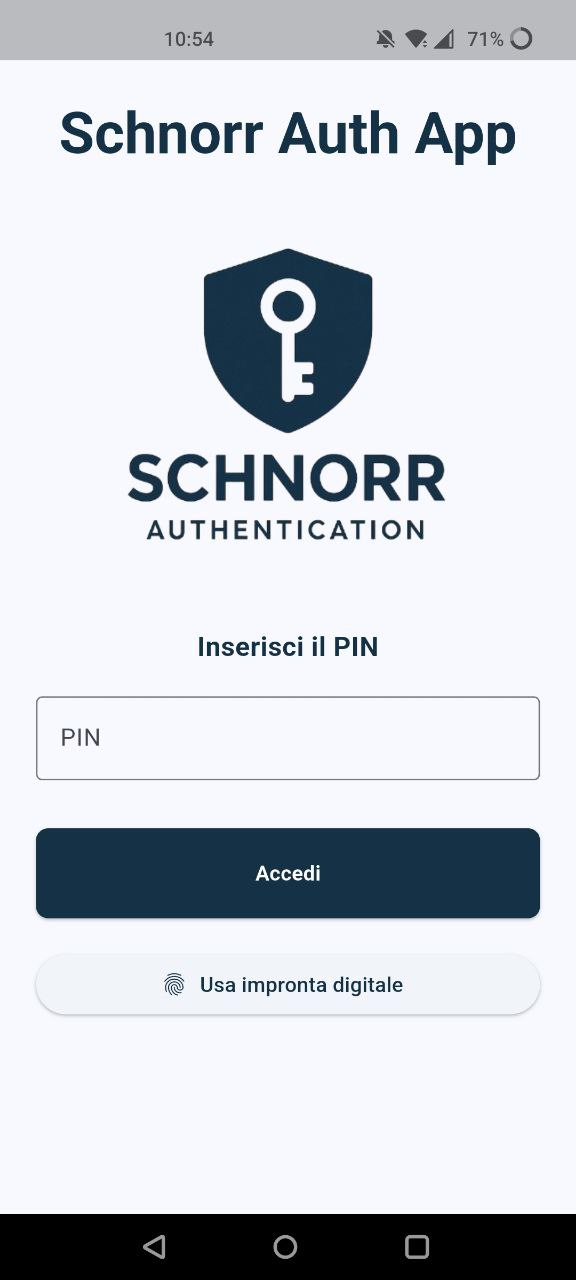
\includegraphics[width=\textwidth]{images/welcome.jpg}
        \caption{Schermata iniziale nella quale impostare il PIN.}
        \label{fig:welcome}
    \end{minipage}\hfill
    \begin{minipage}{0.45\textwidth}
        \centering
        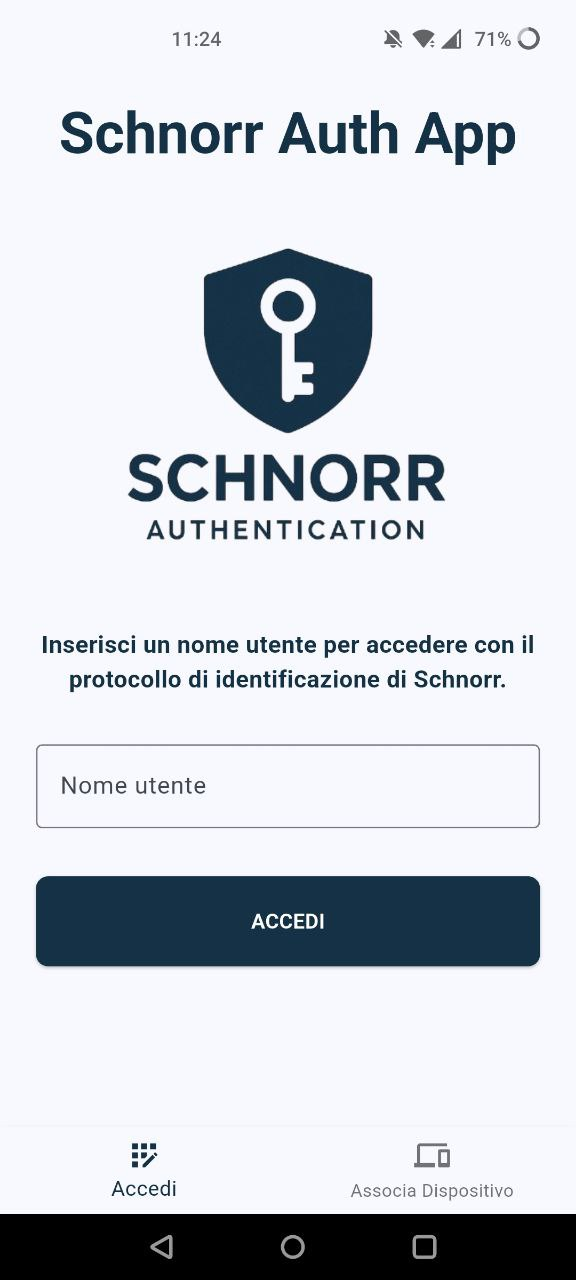
\includegraphics[width=\textwidth]{images/auth.jpg}
        \caption{Fase di registrazione/autenticazione.}
        \label{fig:auth}
    \end{minipage}
\end{figure}

\begin{figure}[h!]
    \centering
    \begin{minipage}{0.45\textwidth}
        \centering
        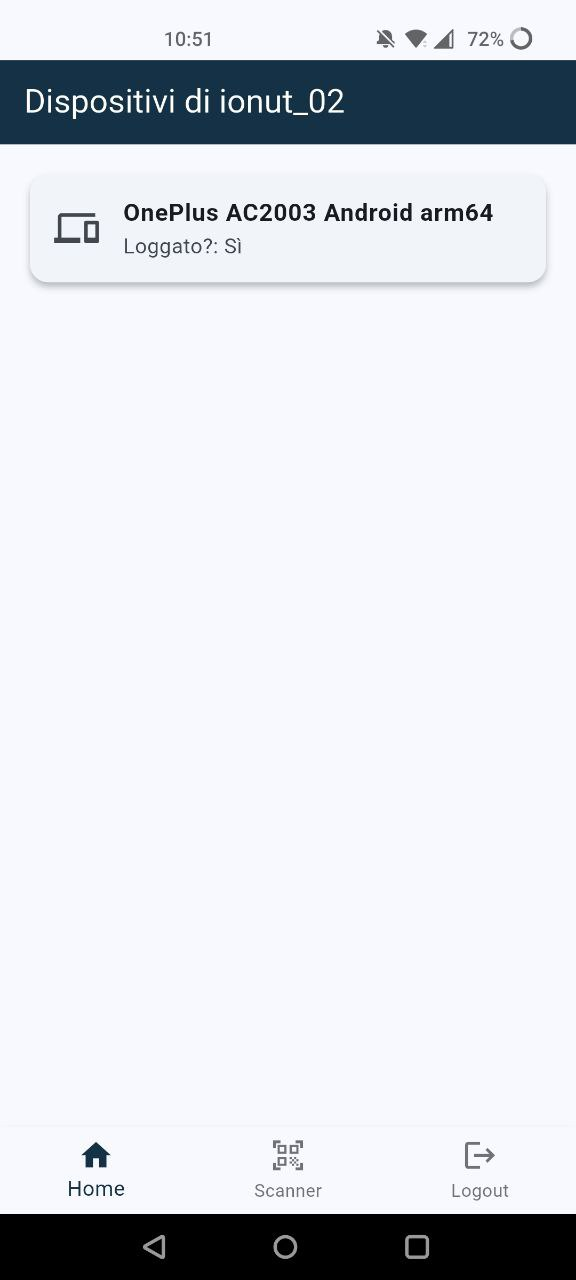
\includegraphics[width=\textwidth]{images/devices.jpg}
        \caption{Pagina principale con dispositivi associati.}
        \label{fig:devices}
    \end{minipage}\hfill
    \begin{minipage}{0.45\textwidth}
        \centering
        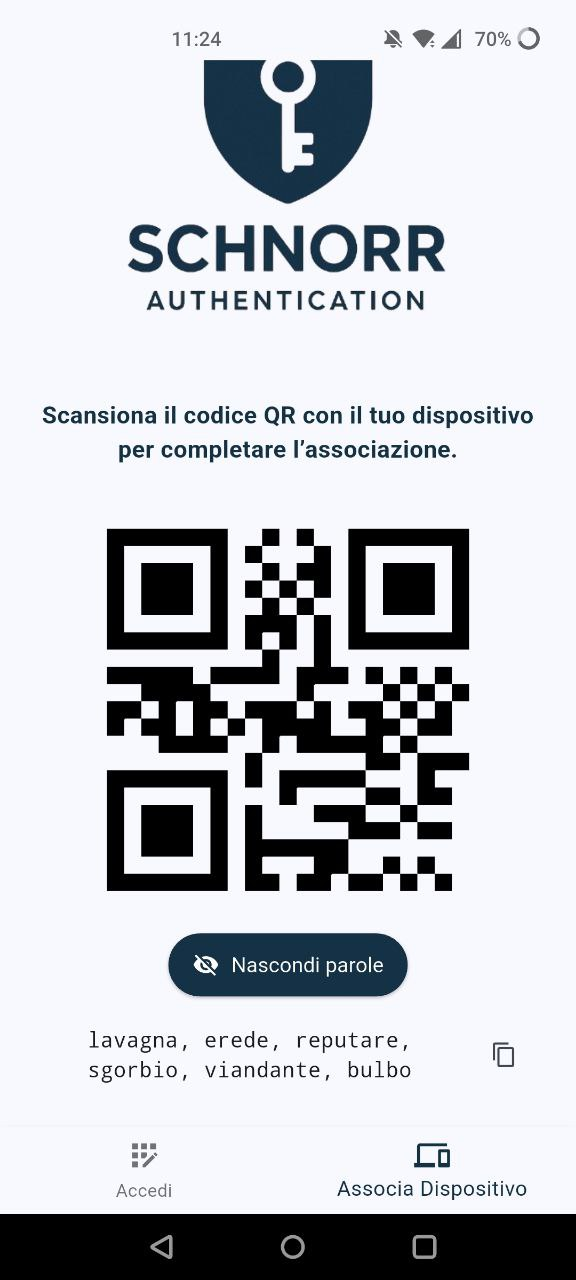
\includegraphics[width=\textwidth]{images/req.jpg}
        \caption{Pagina con QR code e parole.}
        \label{fig:qr_code}
    \end{minipage}
\end{figure}
